\documentclass{homework}
\usepackage{marvosym}
\usepackage{hyperref}

\course{Algorithmische Bioinformatik}
\semester{Wintersemester 2012 / 2013}
\no{6}
\date{Montag, dem 26. November 2012}
\author{Stefan Meißner (4279113) und Niels Hoppe (4356370)}
\tutorial{Dienstag 08:00 - 10:00}
\tutor{Alena van Bömmel (Übungsgruppe 3)}

\begin{document}
\maketitle
\begin{enumerate} 

\aufgabe{Random Sampling}{20}
\begin{enumerate}
\item

\item 
\end{enumerate}

\aufgabe{Verteilungen}{40}
\begin{enumerate}
\item
Wir nutzen die Poisson-Verteilung: \\
$f(x) = P(X=x) = \frac{\mu^x}{x!} e^{-\mu}$ \\ \\
mit $n = 60$, $P = \frac{1}{365}$, $\rightarrow \mu = nP = \frac{12}{73}$\\ \\
Gesucht ist: $P(X \geq 1) = 1 - P(X \leq 0)$ \\
$1-P(X \leq 0) = 1 - \frac{\frac{12}{73}^0}{0!} e^{-\frac{12}{73}} = 1 - 0,8484 = 0,1516$\\ \\
Die Wahrscheinlichkeit dafür, dass von 60 Studenten mindestens einer heute Geburtstag hat beträgt somit 15.16\%.
\item
\end{enumerate}

\aufgabe{Alignment Statistik}{80}

\begin{enumerate}
\item

\begin{lstlisting}[language=python]
import random
import os

N = 10000
LEN = 1000
f = open('library.fa', 'w')
nukl = ['A','C','G','T']

for i in range(N):
    f.write('> random'+str(i)+os.linesep)
    for j in range(LEN):
        f.write(random.choice(nukl))
    f.write(os.linesep)

f.close()
\end{lstlisting}

\item

\begin{lstlisting}[language=python]
import random
import os

K = 100
f = open('query.fa', 'w')
nukl = ['A','C','G','T']

f.write('> myrandomnukl'+os.linesep)

for i in range(K):
    f.write(random.choice(nukl))
    
f.close()
\end{lstlisting}

\begin{lstlisting}[language=python]
query = open('query.fa', 'r')
db = open('library.fa','r')

query_string = query.readlines()[1][:-1]
count = 0

for line in db:
    if( query_string in line):
        ++count

print (count)

query.close()
db.close()
\end{lstlisting}     

Die Sequenz kommt $0$ mal vor.

\item

\begin{verbatim}
       opt      E()
  20     0     0:
  22     0     0:           one = represents 17 library sequences
  24     0     0:
  26     3     0:=
  28     0     2:*
  30    30    14:*=
  32   113    53:===*===
  34   113   144:======= *
  36   565   297:=================*================
  38   627   490:============================*========
  40   504   684:==============================          *
  42  1014   836:=================================================*==========
  44   842   922:==================================================    *
  46   792   939:===============================================        *
  48   836   899:==================================================  *
  50   665   821:========================================        *
  52   602   721:====================================      *
  54   560   616:=================================   *
  56   487   515:============================= *
  58   432   423:========================*=
  60   376   342:====================*==
  62   305   274:================*=
  64   230   218:============*=
  66   198   173:==========*=
  68   133   136:=======*
  70   112   106:======*
  72    88    83:====*=
  74    82    65:===*=
  76    79    50:==*==
  78    53    39:==*=
  80    46    30:=*=
  82    27    23:=*
  84    20    18:=*
  86    12    14:*
  88     8    11:*          inset = represents 1 library sequences
  90     9     9:*
  92     6     7:*         :======*
  94     7     5:*         :====*==
  96     4     4:*         :===*
  98     6     3:*         :==*===
 100     5     2:*         :=*===
 102     3     2:*         :=*=
 104     2     1:*         :*=
 106     2     1:*         :*=
 108     0     1:*         :*
 110     0     1:*         :*
 112     1     1:*         :*
 114     1     0:=         *=
 116     0     0:          *
 118     0     0:          *
 120     0     0:          *
\end{verbatim} 
 
\item siehe (e)
\item 
	R Code zum Erzeugen des Histogramms:
\begin{lstlisting}[language=r]
data <- read.csv("/home/sme/git/albi_w12/data/u6_aufg22_histo.dat",
	header=T, sep='\t')
mean = sum(data[1]*data[2])/10000
variance = sum(((data[1]-mean))^2*data[2])/10000
sigma = sqrt(variance)
data[2] = data[2]/10000
plot(data, type='h', lwd=2)
lines(seq(min(data[1]), max(data[1])),
	dnorm(seq(min(data[1]), max(data[1])), mean, sigma),
	col="blue")
\end{lstlisting}
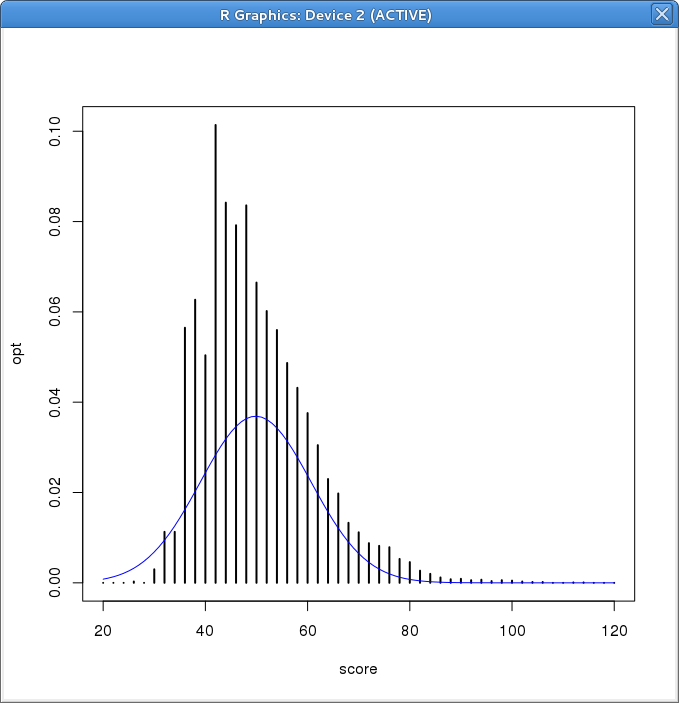
\includegraphics[scale=0.5]{u6_aufg22.png}
\item 
\end{enumerate}

\aufgabe{TATA-Box}{30}

\begin{enumerate}
\item Wir addieren einen pseudo-count von $1$ zu jedem Eintrag der count matrix
$C$ und erhalten so $C'$ mit
$$
C' = \begin{pmatrix}
17 & 353 & 4 & 355 & 269 & 361 & 223\\
47 & 1 & 11 & 1 & 1 & 4 & 3\\
19 & 3 & 3 & 5 & 1 & 21 & 45\\
310 & 36 & 375 & 31 & 122 & 7 & 122
\end{pmatrix}.
$$
Darin ist die Summe aller Beobachtungen pro Spalte $393$. Durch Normierung jedes
Eintrages aus $C'$ mit $\frac{1}{393}$ erhalten wir $P$ mit
$$
P = \begin{pmatrix}
0,043 & 0,898 & 0,010 & 0,903 & 0,684 & 0,919 & 0,567\\
0,12 & 0,003 & 0,028 & 0,003 & 0,003 & 0,010 & 0,008\\
0,048 & 0,008 & 0,008 & 0,015 & 0,003 & 0,053 & 0,115\\
0,789 & 0,092 & 0,954 & 0,079 & 0,310 & 0,18 & 0,310
\end{pmatrix}.
$$
\item Wir berechnen daraus die $PSSM$ mit Einträgen
$PSSM_{i,j} = \log(P_{i,j}, \frac{1}{4})$ als
$$
PSSM = \begin{pmatrix}
-1,754 & 1,279 & -3,201 & 1,285 & 1,007 & 1,301 & 0,82\\
-0,737 & -4,588 & -2,19 & -4,588 & -4,588 & -3,201 & -3,489\\
-1,643 & -3,489 & -3,489 & -2,796 & -4,588 & -1,543 & -0,781\\
1,149 & -1,004 & 1,339 & -1,153 & 0,217 & -2,642 & 0,217
\end{pmatrix}.
$$
Auf Grundlage der auf drei Nachkommastellen gerundeten Werte erhält die Sequenz
\texttt{TATATAT} einen Score von $1,149 + 1,279 + 1,339 + 1,285 + 0,217 + 1,301 + 0,217 = 5,787$.
\end{enumerate}

\end{enumerate}
\end{document}
